%--------------------------------------------------------------------------------------------------
%
\chapter{Nonlinear Multiview Canonical Correlation Analysis}\label{chap:extensions}
%--------------------------------------------------------------------------------------------------

This chapter will discuss generalizations of CCA to
analysis of multiple sets of variables. The
problem is then known as the Multi-set Canonical Correlation Analysis
(MCCA), or sometimes Multiview Canonical Correlation Analysis.
Whereas it can be shown that CCA can be solved using an
(generalized) eigenvalue computation, MCCA is a much more
difficult problem. We will describe a generalization
proposed in~\cite{Kettenring} and present an iterative
locally optimal solution proposed in~\cite{Horst}, referred to
as the \emph{Horst algorithm}, which
represents as a starting point of our work.

For use in practical applications, we propose a novel algorithm based on two original contributions of the Horst algorithm: we adapt the methods to use kernels and to find
multi-dimensional solutions, analogous to finding multiple principal directions
in PCA and multiple pairs of canonical vectors in CCA.

\section{Related Work}\label{chap:extensions:related}
CCA, introduced in Chapter~\ref{chap:background:cca}, was developed to detect linear relations between
two sets of variables. Typical uses of CCA include statistical tests of dependence between two random vectors, exploratory
analysis on multi-view data, dimensionality reduction and finding a common embedding
of two random vectors that share mutual information.

CCA has been generalized in two directions: extending the method to finding nonlinear
relations  by using kernel methods~\cite{FBMJ}\cite{HardoonCCA} and extending the 
method to more than two sets of variables which was introduced in~\cite{Kettenring} which
we presented in~\ref{chap:background:kernels}.
Among several proposed generalizations in \cite{Kettenring} the most important for our work are the \emph{Sum
of Correlations} (SUMCOR) and \emph{Sum of Squared Correlations} (SSCOR) generalizations, where SUMCOR
will be the main focus of the current chapter and the Chapter~\ref{chap:extensions} and SSCOR will
be studied in Chapter~\ref{chap:crosslingual}.

There the goal is to project $m$ sets of random variables to $m$ univariate random variables,
which are pair-wise highly correlated on average
\footnote{Given $m$ univariate random variables, one can compute $\binom{m}{2}$ correlation
coefficients, one for each pair of variables.}.
An iterative method to solve the SUMCOR generalization was proposed in \cite{Horst}
and the proof of convergence was established in \cite{Chu}. In \cite{Chu} it was shown
that a generic SUMCOR problem admits exponentially many locally optimal solutions. 
In \cite{GlobalMEP2} the authors identified a subset of SUMCOR problems for which the iterative
procedure converges to a global maximizer (Their results apply to nonnegative irreducible quadratic forms).
In Chapter~\ref{chap:relaxations} we will discuss results on the problem complexity and global optimality
conditions.

This chapter will focus on the local iterative approach~\cite{Horst} with the aim of extending it
so it may be used in applications similar to KCCA.
Here we show how the method can be extended to finding non-linear patterns and finding more than one
set of canonical variates. Our work is related to \cite{JointBSSAppl} where a deflation scheme
is used together with the Newton method to find several sets of canonical variates.
Our nonlinear generalization is related to \cite{nonlinJointBSS}, where the main difference
lies in the fact that we "kernelized" the problem, whereas the authors in \cite{nonlinJointBSS}
worked with explicit nonlinear feature representation.

We now list some applications of the SUMCOR formulation. In \cite{kernelHyperAppl} an optimization
problem for multi-subject functional magnetic resonance imaging (fMRI) alignment is proposed,
which can be formulated as a SUMCOR problem (performing whitening on each set of variables).
Another application of the SUMCOR formulation can be found in \cite{JointBSSAppl}, 
where it is used for group blind source separation on fMRI data from multiple subjects.
An optimization problem equivalent to SUMCOR also arises in control theory \cite{ControlApplication}
in the form of linear sensitivity analysis of systems of differential equations.

\section{Sum of Correlations}\label{chap:extensions:sumcor}

In this section we will discuss a generalization of CCA to more than two views,
which finds a set of directions (one per view) which maximizes the average correlation
(computed for each pair of views).

We assume that we are given a centered random vector $\mathcal{X} \in \RR^N$ as defined in~\ref{def:notation:multiview_dataset},
where $\mathcal{X}$ is composed of $m$ subsets of random variables referred to as views. We assume that the indices of components
of each set are contiguous, i.e. $\mathcal{X}$ is a concatenation of blocks that correspond to views.

\noindent\textbf{Additional Notation.}
Let $m$ denote the number of blocks and $N$ the total number of
variables in $\mathcal{X}$. Then
$$b := \left(n_1, \ldots, n_m\right), \sum_{i=1}^m b\left(i\right) = N$$
encodes the number of elements in each of the block. We denote the corresponding
sub-vectors as $\mathcal{X}^{(i)} \in \RR^{n_i}$
($i$-th block-row of vector $\mathcal{X}$) and the sub-matrices as $C^{(i,j)} \in \RR^{n_i \times n_j}$
($i$-th block-row, $j$-th block column of matrix $C$); see Figure~\ref{fig:block_structure}.
For example, in CCA, there are only two sets, so $m=2$.
\begin{figure}[t]
\centering
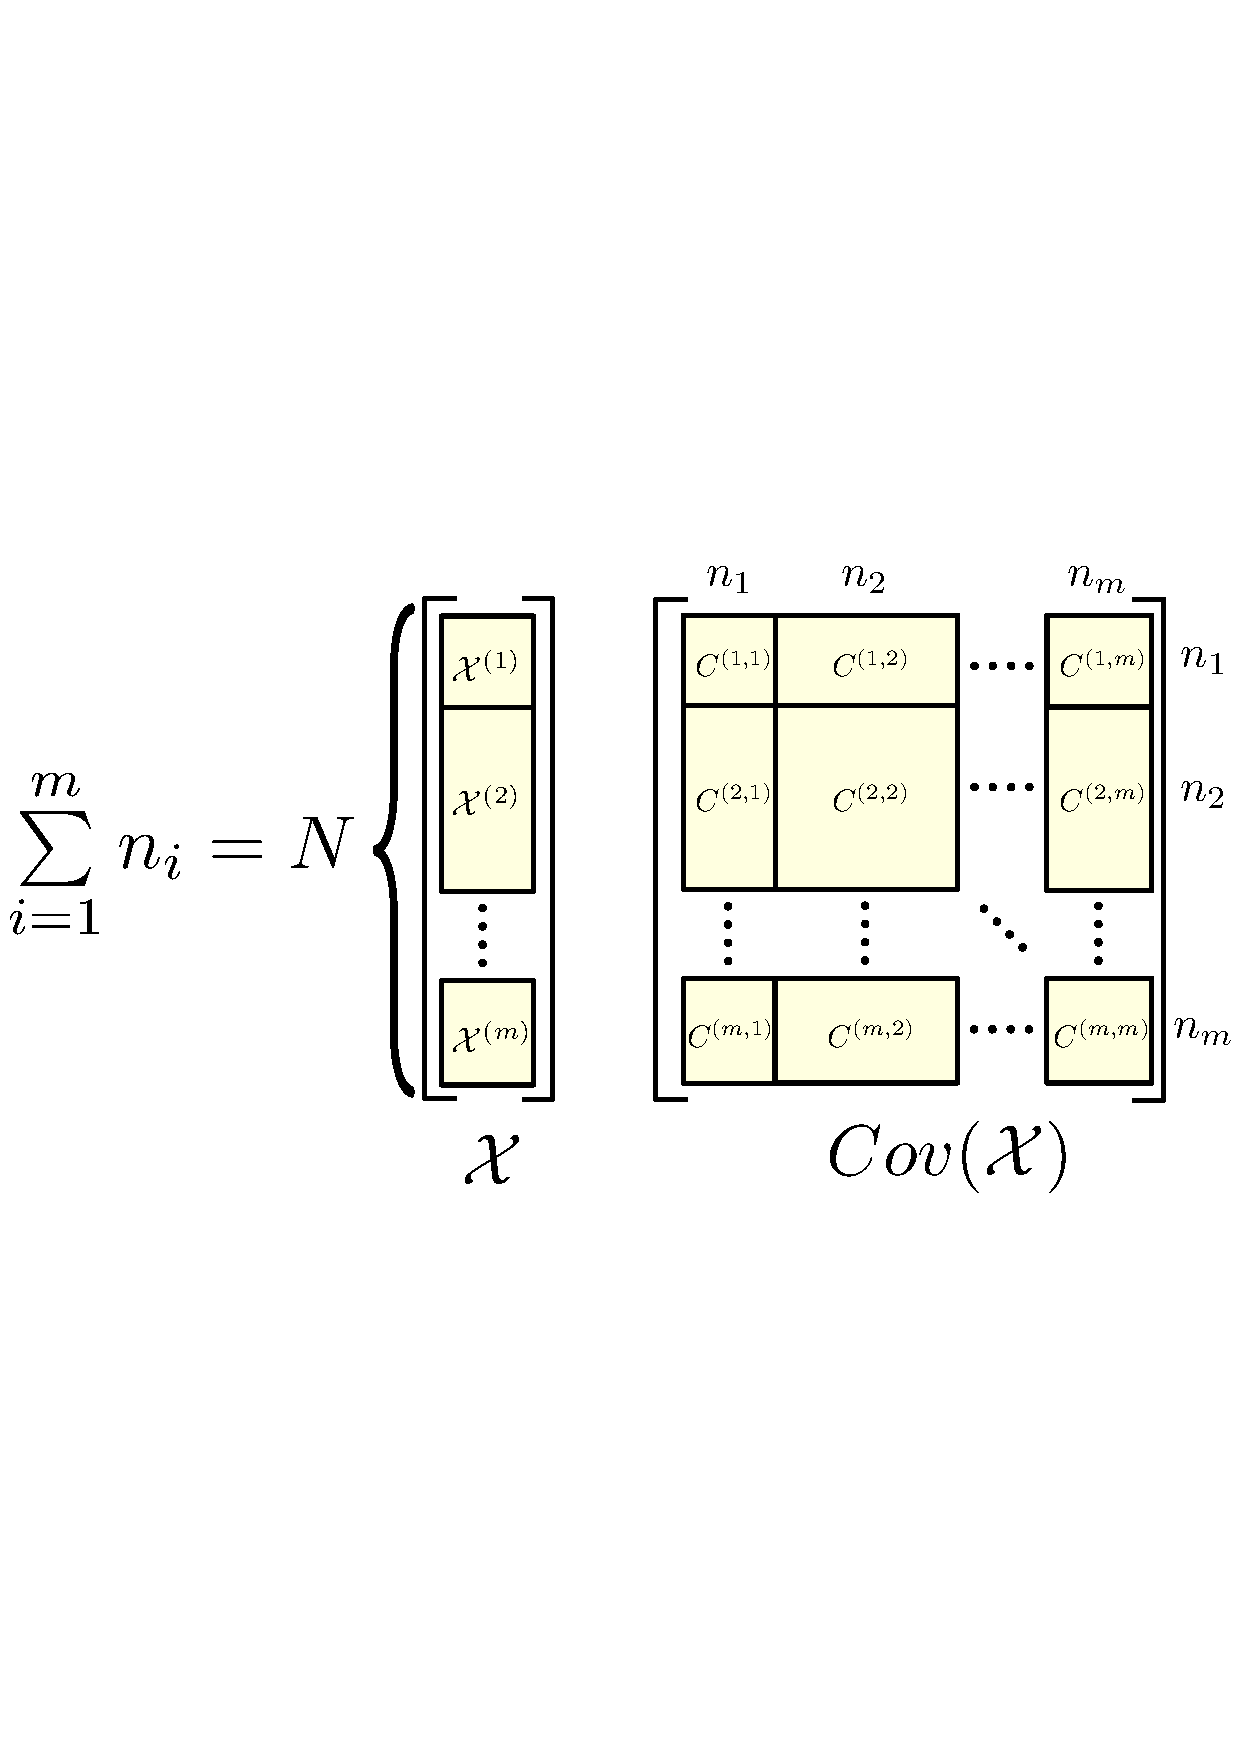
\includegraphics[width=0.5\textwidth]{figures/block_structure.pdf}
\caption{\label{fig:block_structure} The block structure of the  random vector $\mathcal{X}$ and the corresponding covariance block structure.}
\end{figure}

Formally, given $w \in \RR^N$ we define $m$ random variables $\mathcal{Z}_i$ (one-dimensional
projections of random block components of $\mathcal{X}$) as:
\begin{equation*}
\mathcal{Z}_i := \sum_{j = 1}^{n_i} \mathcal{X}^{(i)}\left(j\right)
w^{(i)}\left(j\right) = \mathcal{X}^{(i)T} \cdot w^{(i)}.
\end{equation*}

Let $\rho\left(x,y\right)$ denote the correlation
 coefficient between two random variables:
\begin{equation*}
\rho\left(x,y\right) =
 \frac{Cov\left(x,y\right)}{\sqrt{Cov\left(x,x\right) Cov\left(y,y\right)}}.
\end{equation*}
 The correlation coefficient between $\mathcal{Z}_i$ and
 $\mathcal{Z}_j$ can be expressed as:
\begin{equation*}
\rho\left(\mathcal{Z}_i, \mathcal{Z}_j\right) = \frac{w^{(i)T} C^{(i,j)}
   w^{(j)}}{\sqrt{w^{(i)T} C^{(i,i)} w^{(i)}}\sqrt{w^{(j)T}
     C^{(j,j)} w^{(j)}} }.
\end{equation*}

\noindent\textbf{Initial Problem Formulation.}

The problem described above can be stated as
finding the set of vectors $w^{(i)}$
which maximize
\begin{equation}\label{eq:SUMCOR}
\tag{SUMCOR}
\sum_{i = 1}^m \sum_{j = i+1}^m
\rho\left(\mathcal{Z}_i, \mathcal{Z}_j\right).
\end{equation}
We refer to this problem as Multi-set Canonical
Correlation Analysis (MCCA). Note that it reduces to CCA when
$m=2$. The solution - that is, the set of components $\left(w^{(1)}, \ldots, w^{(m)}\right)$,
are referred to as the set of canonical vectors.

Another formulation proposed in~\cite{Kettenring} is the \emph{Sum of Squared Correlations} (SSCOR)
\begin{equation}\label{eq:SSCOR}
\tag{SSCOR}
\sum_{i = 1}^m \sum_{j = i+1}^m
\rho\left(\mathcal{Z}_i, \mathcal{Z}_j\right)^2.
\end{equation}
The second formulation is invariant to the signs of the correlation coefficients. It will
be of importance in Chapter~\ref{chap:crosslingual}.

\noindent\textbf{Reformulating the Optimization Problem.}
Expanding SUMCOR, we get:

\begin{equation*}
\begin{aligned}
& \underset{w \in \RR^N}{\text{max}} & & \sum_{i = 1}^m
  \sum_{j = i+1}^m \frac{w^{(i)T} C^{(i,j)}
    w^{(j)}}{\sqrt{w^{(i)T} C^{(i,i)} w^{(i)}} \sqrt{w^{(j)T}
      C^{(j,j)} w^{(j)}}}.
\end{aligned}
\end{equation*}

Observe that the solution is invariant to scaling (only the direction matters):
if $\left(w^{(1)}, \ldots, w^{(m)}\right)$ is a solution, then
$\left(\alpha_1 \cdot w^{(1)}, \ldots, \alpha_m \cdot w^{(m)}\right)$ is also a
solution for $\alpha_i > 0$. We may therefore impose constraints $w^{(i)T}C^{(i,i)}w^{(i)} = 1$,
which only affect the norm. This yields the following  equivalent constrained problem:
\begin{equation}\label{eq:qcqp0}
\begin{aligned}
& \underset{w \in \RR^N}{\text{maximize}}
& & \sum_{i = 1}^m \sum_{j = i+1}^m w^{(i)T} C^{(i,j)} w^{(j)}\\
& \text{subject to}
& &w^{(i)T} C^{(i,i)} w^{(i)} = 1, \quad\forall i = 1,\ldots, m.
\end{aligned}
\end{equation}
We further multiply the objective by $2$ and add a constant $m$. Note that this does not
affect the optimal solution. Using the equalities: $w^{(i)T} C^{(i,j)} w^{(j)} = w^{(j)T} C^{(j,i)} w^{(i)}$
and $w^{(i)T} C^{(i,i)} w^{(i)} = 1$, we obtain:

\begin{equation}\label{eq:qcqp05}
\begin{aligned}
& \underset{w \in \RR^N}{\text{maximize}}
& & \sum_{i = 1}^m \sum_{j = 1}^m w^{(i)T} C^{(i,j)} w^{(j)}\\
& \text{subject to}
& &w^{(i)T} C^{(i,i)} w^{(i)} = 1, \quad\forall i = 1,\ldots, m.
\end{aligned}
\end{equation}
This transforms the objective function into a quadratic form $w^T C w$. To
simplify the constraints, assume that $C^{(i,i)}$ is strictly positive definite.
If $C^{(i,i)}$ is not full rank, then using the eigenvalue decomposition
$C^{(i,i)} = V \Lambda V^T$, where $V \in \RR^{n_i \times k}$,
$\Lambda \in \RR^{n_i \times k}$, $\Lambda > 0$, $k < n_i$,
we substitute $\mathcal{X}^{(i)}$ with $V^T \mathcal{X}^{(i)} \in \RR^k$,
for which the covariance matrix is strictly positive definite.

From the strict positive definiteness it follows that $C^{(i,i)}$ admits a Cholesky
decomposition: there exists an invertible matrix $D_i$ such that $C^{(i,i)} = D_i^T D_i$.

Finally, using the block structure $b$, we substitute $w^{(i)}$
with $D_i^{-1} x^{(i)}$ and define $A \in \RR^N$ as:
\begin{equation*}
A^{(i,j)} := {D_i}^{-T} C^{(i,j)} {D_j}^{-1},
\end{equation*}
leading to the simplified problem:
 \begin{equation}\label{eq:qcqp}
\tag{QCQP}
\begin{aligned}
& \underset{x \in \RR^{N}}{\text{max}}
& & x^T A x\\
& \text{subject to}
& &x^{(i)T} x^{(i)} = 1, \quad\forall i = 1, \ldots, m.
\end{aligned}
\end{equation}
It turns out that (\ref{eq:qcqp}) is simpler to  manipulate than  (\ref{eq:SUMCOR}), so we use this form from this point on.

\section{Local Solutions}\label{chap:extensions:horst}
In this section, we give an algorithm that converges to a locally optimal
solutions of the problem (\ref{eq:qcqp}), when the matrix $A$ is symmetric,
positive-definite and generic (the proof was established in \cite{Chu}).

The algorithm can be interpreted as a generalization of the power
iteration method (also known as the Von Mises iteration), a classical
approach to finding the largest solutions to the eigenvalue problem
$A x = \lambda x$.  The general iterative procedure is given
as Algorithm~\ref{algorithm:horst}.
\begin{algorithm}
\caption{Horst algorithm}
\label{algorithm:horst}
{\bf Input:} matrix $A \in \sym_N^+$, block structure $b = \left(n_1,\ldots,n_m\right)$,
initial vector $x_0 \in \RR^N$ with $\norm{x^{(i)}} > 0$,  \par
\begin{algorithmic}
\STATE $x \leftarrow x_0;$
\FOR{$iter = 1$ to $maxiter$}
\STATE $x \leftarrow A x;$
\FOR{$i =1$ to $m$}
\STATE $x^{(i)} \leftarrow \frac{x^{(i)}}{\norm{x^{(i)}}}$
\ENDFOR
\ENDFOR
\end{algorithmic}
{\bf Output:} $x$
\end{algorithm}

In the case of $m=1$,  Algorithm~\ref{algorithm:horst}
corresponds exactly to the power iteration. While the algorithm's
convergence is guaranteed, its convergence rate is not known. In
Chapter~\ref{chap:experiments} we will examine the convergence
rate on synthetic data.

\section{Proposed Extensions}

Here we present two extensions of MCCA: how to use kernel methods with
MCCA to find nonlinear dependencies in the data; and an
algorithm to finding more then one set of correlation vectors.
\subsection{Dual Representation and Kernels}\label{chap:extensions:kernels}

We return to formulation (\ref{eq:qcqp0}):
\begin{equation*}
\begin{aligned}
& \underset{w \in \RR^N}{\text{max}}
& & \sum_{i = 1}^m \sum_{j = i+1 }^m w^{(i)T} C^{(i,j)} w^{(j)}\\
& \text{subject to}
& &w^{(i)T} C^{(i,i)} w^{(i)} = 1, \quad\forall i = 1,\ldots, m,
\end{aligned}
\end{equation*}
where $b = \left(n_1,\ldots,n_m\right)$ denotes the block structure
and $ \sum_i n_i = N $.
In the previous sections, we focused on manipulating covariance matrices
only and omitted details on their estimation based on finite samples.
In this section, we will use a formulation that explicitly presents
the empirical estimates of covariances, which will enable us to apply kernel methods.
Let $\mathcal{X}$ be a random vector distributed over $\RR^N$ with
$E\left(\mathcal{X}\right) = 0$. Let $X \in \RR^{N \times s}$
represent a sample of $s$ observations of $\mathcal{X}$, where each
observation corresponds to a column vector. The empirical covariance of $\mathcal{X}$
based on the sample matrix $X$ is expressed as:
$$ \overline{Cov\left(\mathcal{X}\right)} = \frac{1}{s - 1}X X^T.$$
If $s < N$, then $\overline{Cov\left(\mathcal{X}\right)}$ is singular which
makes the optimization problem ill-posed and may lead to overfitting
(discovering spurious patterns in the data). These issues are addressed by
using regularization techniques, typically a shrinkage estimator
$\overline{Cov\left(\mathcal{X}\right)_{\kappa}}$ is defined as:
$$ \overline{Cov\left(\mathcal{X}\right)_{\kappa}} = \left(1-\kappa\right)
 \frac{1}{s - 1}X X^T + \kappa  I_N,$$ where $\kappa \in \left[0,1\right]$.

Using the block structure $b$, (\ref{eq:qcqp05}) becomes:
 \begin{equation}\label{eq:regqcqp}
\begin{aligned}
& \underset{w \in \RR^N}{\text{max}}
& & \frac{1}{s -1} \sum_{i = 1}^m \sum_{j = i+1}^m w^{(i)T} X^{(i)}X^{(j)T} w^{(j)} \\
& \text{subject to}
& & w^{(i)T} \left(\frac{1- \kappa}{s - 1}X^{(i)} X^{(i)T} + \kappa  I_N\right) w^{(i)} = 1,\\&&& \quad\forall i = 1,\ldots, m.
\end{aligned}
\end{equation}
To express each component $w^{(i)}$ in terms the columns of $X^{(i)}$,
let $w$ have block structure $b_w = \left(n_1, \ldots, n_m\right)$
where $\sum_i n_i = N$, and let $y \in \RR^{m\cdot s}$ have block
structure $b_y\left(i\right) = s, \forall i = 1,\ldots, m$. The
component $w^{(i)}$ can be expressed as:
\begin{equation}\label{eq:representer}
\begin{aligned}
w^{(i)} = \sum_{j = 1}^{s} y^{(i)}\left(j\right) X^{(i)}\left(:,j\right) = X^{(i)} y^{(i)}.
\end{aligned}
\end{equation}
We refer to $y$ as dual variables.

It remains to check that the formulations (\ref{eq:regqcqp}) and (\ref{eq:dualregqcqp})
are equivalent.
\begin{lemma}
There exists a solution to \eqref{eq:regqcqp} which can be expressed as \eqref{eq:representer}.
\end{lemma}
\begin{proof}
We prove the lemma by contradiction. Assume that no optimal solution
can be expressed as \eqref{eq:representer} and $u$ be an optimal solution to the
problem \eqref{eq:regqcqp}. Without loss of generality, assume
that $u^{(1)}$ does not lie in the column space of $X^{(1)}$:
 $$u^{(1)} = z_{\bot} + X^{(1)} y^{(1)},$$
 where $$z_{\bot} \neq 0_{n_1}\quad \text{and}\quad X^{(1)T}z_{\bot} = 0_s.$$
We show that $\bar{u}$, defined as $\bar{u}^{(i)} := u^{(i)}, \forall i> 1$
and $\bar{u}^{(1)} := \frac{1}{\gamma}  X^{(1)} y^{(1)},$ where
\begin{equation*}
\gamma :=\sqrt{ y^{(1)T} X^{(1)T} \left(\frac{1- \kappa}{s - 1}X^{(1)} X^{(1)T} + \kappa  I_N\right) X^{(1)} y^{(1)} },
\end{equation*}
strictly increases the objective function, which contradicts the assumption
that $u$ is optimal. Clearly, $\bar{u}$ is a feasible solution. Positive
definiteness of $\frac{1- \kappa}{s - 1}X^{(1)} X^{(1)T} + \kappa  I_N$,
coupled with the fact that $z_{\bot}^T z_{\bot} > 0$ implies that
$0 < \gamma < 1$. Let $E := \sum_{j = 2}^m \left(X^{(1)} y^{(1)}\right)^T X^{(1)}X^{(j)T} u^{(j)}$.

If $E < 0$, then the vector $[-u^{(1)T} u^{(2)T} \cdots u^{(m)T}]^T$ strictly increases the
objective function, which is a contradiction. We also obtain a contradiction if $E = 0$,
since any nonzero $v \in \RR^{s}$ for which $X^{(1)}v \neq 0_{n_1}$ can be used to obtain
a solution to the problem \eqref{eq:regqcqp} expressed as \eqref{eq:representer}
(after re-scaling  such that $\overline{Cov\left(\mathcal{X}^{(1)}v\right)_\kappa} = 1$
and if necessary multiplying it by $-1$ so that $\sum_{j = 2}^m \left(X^{(1)} v\right)^T X^{(1)}X^{(j)T} u^{(j)}) \geq 0$).
Thus, we may assume that $E > 0$.

The following inequality completes the proof, since it shows that $\bar{u}$ increases the objective function:

\begin{align*}
  \frac{1}{s -1} & \sum_{j = 2}^m u^{(1)T} X^{(1)}X^{(j)T} u^{(j)} =\\
= \frac{1}{s -1} & \sum_{j = 2}^m \left(z_{\bot} + X^{(1)} y^{(1)}\right)^T X^{(1)}X^{(j)T} u^{(j)} = \\
= \frac{1}{s -1}  &\sum_{j = 2}^m \left(X^{(1)} y^{(1)}\right)^T X^{(1)}X^{(j)T} u^{(j)} < \\
< \frac{1}{s -1}  &\sum_{j = 2}^m \frac{1}{\gamma}\left(X^{(1)} y^{(1)}\right)^T X^{(1)}X^{(j)T} u^{(j)}.
\end{align*}
\end{proof}

Let $K_i = X^{(i)T} X^{(i)} \in \RR^{s \times s}$ denote the Gram
matrix. Next, we express the problem (\ref{eq:regqcqp}) in terms of the dual variables:
 \begin{equation}\label{eq:dualregqcqp}
\begin{aligned}
& \underset{y \in \RR^{m\cdot s}}{\text{max}}
& & \frac{1}{s -1} \sum_{i = 1}^m \sum_{j = i+1}^m y^{(i)T} K_i K_j^T y^{(j)} \\
& \text{subject to}
& & y^{(i)T} \left(\frac{1- \kappa}{s - 1}K_i K_i^T + \kappa  K_i\right) y^{(i)} = 1,\\
& &&\quad\forall i = 1,\ldots, m.
\end{aligned}
\end{equation}
Expressing the problem in terms of Gram matrices makes it amenable to using kernel methods (see \cite{shawe-taylor04kernel}).

Typically the matrices $K_i$ are ill conditioned (or even singular
when the data is centered) and it is advantageous to constrain the
magnitude of dual coefficients as well as the variance in the original
problem. We address this by introducing a first order approximation to
the dual regularized variance. Let
$$\widetilde{K_i} := \left(\sqrt{\frac{1-\kappa}{s - 1}}K_i + \frac{\kappa}{2}
  \sqrt{\frac{s-1}{1- \kappa}}I_s\right).$$
The covariance becomes:
$$ \overline{Cov\left(\mathcal{X}^{(i)}\right)_{\kappa}} =
 \frac{1- \kappa}{s - 1}K_i K_i^T + \kappa  K_i \approx  \widetilde{K_i} \widetilde{K_i}^T.$$
This approximation has two advantages: it is invertible and is in a
factorized form. We exploit the latter when obtaining a convergent local method.
The final optimization is then expressed as:
 \begin{equation}\label{eq:approxdualqcqp}
\begin{aligned}
& \underset{y \in \RR^{m\cdot s}}{\text{max}}
& & \frac{1}{s - 1} \sum_{i = 1}^m \sum_{j = i+1}^m y^{(i)T} K_i K_j^T y^{(j)}\\
& \text{subject to}
& & y^{(i)T} \widetilde{K_i} \widetilde{K_i}^T y^{(i)} = 1, \quad\forall i = 1,\ldots, m.
\end{aligned}
\end{equation}

The problem can be interpreted as maximizing covariance while constraining variance
and magnitude of dual coefficients.

\subsection{Computing Several Sets of Canonical Vectors}\label{chap:extensions:severalCanonicalVectors}
Usually a one-dimensional representation does not sufficiently capture
all the information in the data and higher dimensional subspaces are
needed. After computing the first set of primal canonical vectors we
proceed to computing the next set. The next set should be almost as
highly correlated as the first one, but essentially ``different'' from
the first one. We achieve this by imposing additional constraints for
every view. Namely, all projection vectors in view $i$ are
uncorrelated with respect to $\widetilde{K}_i^2$ (this is similar to
the approach in two view regularized kernel CCA\cite{FBMJ}).
\par
Let $Y = \left[y_1, \ldots, y_k\right] \in \RR^{m\cdot s  \times k}$
represent $k$ sets of canonical vectors, where
$$Y^{(\ell)T} \widetilde{K_{\ell}^2} Y^{(\ell)} = I_k  \quad\forall \ell = 1,\ldots, m. $$
The equation above states that each canonical vector has unit regularized variance 
and that different canonical vectors corresponding to the same view are
uncorrelated (orthogonal with respect to $\widetilde{K_i^2}$).

We will now extend the set of constraints in the optimization (\ref{eq:approxdualqcqp})
to enforce the orthogonality.

 \begin{equation}\label{eq:kdimapproxdualqcqp}
\begin{aligned}
& \underset{y \in \RR^{m\cdot s}}{\text{max}}
& & \frac{1}{s -1} \sum_{i = 1}^m \sum_{j = i+1}^m y^{(i)T} K_i K_j^T y^{(j)}\\
& \text{subject to}
& & y^{(i)T} \widetilde{K_i} \widetilde{K_i}^T y^{(i)} = 1, \quad\forall i = 1,\ldots, m\\
& & & Y^{(i)T} \widetilde{K_i} \widetilde{K_i}^T y^{(i)} = 0_k, \quad\forall i = 1,\ldots, m.
\end{aligned}
\end{equation}

To use the Horst algorithm, we first use the substitutions:
$$Z^{(i)} = \widetilde{K_i}Y^{(i)}, \quad z^{(i)} = \widetilde{K_i}y^{(i)}$$
and define the operators $$P_i = I_s - \widetilde{K}_i Y^{(i)} Y^{(i)T} \widetilde{K}_i = I_s - Z^{(i)} Z^{(i)T},$$
which map to the space orthogonal to the columns of $\widetilde{K}_i Y^{(i)}$.
Each $P_i$ is a projection operator: $P_i^2 = P_i,$ which follows directly from the identities above.
The optimization problem in the new variables is:

 \begin{equation}\label{eq:Zkdimapproxdualqcqp}
\begin{aligned}
& \underset{z \in \RR^{m\cdot s}}{\text{max}}
& & \frac{1}{s -1} \sum_{i = 1}^m \sum_{j = i+1}^m z^{(i)T} \widetilde{K_i}^{-T} K_i K_j^T \widetilde{K_j}^{-1} z^{(j)} \\
& \text{subject to}
& & z^{(i)T}  z^{(i)} = 1, \quad\forall i = 1,\ldots, m\\
& & & Z^{(i)T} z^{(i)} = 0_k, \quad\forall i = 1,\ldots, m.
\end{aligned}
\end{equation}

Using the projection operators, this is equivalent to:
\begin{equation*}
\begin{aligned}
& \underset{z \in \RR^{m\cdot s}}{\text{max}}
& & \frac{1}{s -1} \sum_{i = 1}^m \sum_{j = i+1}^m z^{(i)T} P_i^T \widetilde{K_i}^{-T} K_i K_j^T \widetilde{K_j}^{-1} P_j z^{(j)}\\
& \text{s.t.}
& & z^{(i)T}  z^{(i)} = 1, \quad\forall i = 1,\ldots, m.
\end{aligned}
\end{equation*}

By multiplying the objective by $2$ (due to the symmetries of $P_i, K_i$ and $\widetilde{K_i}$)
and shifting the objective function by $\frac{m}{1 - \kappa}$, the problem is equivalent to:
\begin{equation}
\begin{aligned}
& \underset{z \in \RR^{m\cdot s}}{\text{max}}
& & \frac{1}{s -1} \sum_{i = 1}^m \sum_{\substack{j = 1\\ j\neq i}}^m z^{(i)T} P_i^T \widetilde{K_i}^{-T} K_i K_j^T \widetilde{K_j}^{-1} P_j z^{(j)}\\
&&& + \frac{1}{1-\kappa}\sum_{i = 1}^m z^{(i)T}  z^{(i)}\\
& \text{s.t.}
& & z^{(i)T}  z^{(i)} = 1, \quad\forall i = 1,\ldots, m.
\end{aligned}
\end{equation}

This optimization can be reformulated as:
\begin{equation}\label{eq:projZkdimapproxdualqcqp}
\begin{aligned}
& \underset{z \in \RR^{m\cdot s}}{\text{max}}
& & z^T A z\\
& \text{subject to}
& & z^{(i)T}  z^{(i)} = 1, \quad\forall i = 1,\ldots, m,
\end{aligned}
\end{equation}
where $A \in \RR^{m\cdot s}$ with block structure $b\left(i\right) = s, \forall i = 1,\ldots, m$, defined by:
\begin{equation*}
 A^{(i,j)} = \left\{ \begin{array}{lll}
 \frac{1}{s -1} P_i^T \widetilde{K_i}^{-T} K_i K_j^T \widetilde{K_j}^{-1} P_j  & {\rm for} ~i \neq j\\
\frac{1}{1-\kappa } I_s & {\rm for} ~i = j \end{array}\right\}.
\end{equation*}

\begin{lemma}
The block matrix $A$ defined above is positive semidefinite (i.e. $A \in \sym_+^{m\cdot s}$).
\end{lemma}
\begin{proof}
$A$ is symmetric, which follows from $P_i = P_i^T$ and $K_i =
K_i^T$. Let $z \in \RR^{m\cdot s}$.  The goal is to show that $z^T A z > 0$.
Let us define an auxiliary matrix $W$ as:
\begin{equation*}
\begin{aligned}
W =  \frac{1}{1- \kappa }&\sum_{i = 1}^m z^{(i)T} P_i^T
\widetilde{K_i}^{-T} \cdot \\&\left( \kappa K_i + \frac{\kappa^2
    \left(s-1\right)}{4\left(1-\kappa\right)}I_s   \right)
\widetilde{K_i}^{-1} P_i z^{(i)}
\end{aligned}
\end{equation*}
Each summand is positive-semidefinite, i.e. $W \geq 0$ and $W > 0$ if $\exists i: P_i z^{(i)} = z^{(i)}$.
What follows is a sequence of inequalities, some of which must be strict, as will be established:
\begin{align}
z^T A z &=  \frac{1}{s -1} \sum_{i = 1}^m \sum_{\substack{j = 1\\j\neq i}}^m z^{(i)T} P_i^T \widetilde{K_i}^{-T} K_i K_j^T \widetilde{K_j}^{-1} P_j z^{(j)}\nonumber
\\& \qquad + \frac{1}{1- \kappa }\sum_{i = 1}^m z^{(i)T}  z^{(i)} \label{proof_line_1}\\
%
&\geq \frac{1}{s -1} \sum_{i = 1}^m \sum_{\substack{j = 1\\ j\neq i}}^m z^{(i)T} P_i^T \widetilde{K_i}^{-T} K_i K_j^T \widetilde{K_j}^{-1} P_j z^{(j)}\nonumber\\
& \qquad + \frac{1}{1- \kappa }\sum_{i = 1}^m z^{(i)T} P_i^T P_i z^{(i)}  \label{proof_line_2}\\
%
 &= \frac{1}{s -1} \sum_{i = 1}^m \sum_{\substack{j = 1\\ j\neq i}}^m z^{(i)T} P_i^T \widetilde{K_i}^{-T} K_i K_j^T \widetilde{K_j}^{-1} P_j z^{(j)}\nonumber\\
 & \qquad+ \frac{1}{1- \kappa }\sum_{i = 1}^m z^{(i)T} P_i^T \widetilde{K_i}^{-T}  \widetilde{K_i}^T \widetilde{K_i} \widetilde{K_i}^{-1} P_i z^{(i)}  \label{proof_line_3}\\
%
&= \frac{1}{s -1} \sum_{i = 1}^m \sum_{\substack{j = 1\\ j\neq i}}^m z^{(i)T} P_i^T \widetilde{K_i}^{-T} K_i K_j^T \widetilde{K_j}^{-1} P_j z^{(j)}\nonumber
\\& \qquad+ \frac{1}{s-1}\sum_{i = 1}^m z^{(i)T} P_i^T \widetilde{K_i}^{-T}  K_i K_i^T \widetilde{K_i}^{-1} P_i z^{(i)} + W  \label{proof_line_4}\\
%
&= z^T B B^T z + W \geq 0\nonumber,
\end{align}
where $B \in \RR^{m\cdot s \times s}$, defined by $B^{(i)} = \frac{1}{\sqrt{s-1}}(K_i \widetilde{K_i}^{-1}P_i)^T$,
with corresponding row block structure $b\left(i\right) = s$. The inequality after (\ref{proof_line_1}) holds
since projection operators cannot increase norms.
(\ref{proof_line_3}) is equal to (\ref{proof_line_2}) using $\widetilde{K_i}^{-T}  \widetilde{K_i}^T = I$.
Regrouping the terms and applying the definition of $W$, we obtain (\ref{proof_line_4}).
The final equality follows, since the first two sums form a perfect square.

Now we will show that at least one of the two inequalities is strict.
If $P_i z^{(i)} \neq z^{(i)}$ for some $i$, then the first inequality is
strict ($\norm{P_i z^{(i)}} < \norm{z^{(i)}}$). Conversely, if $P_i z^{(i)} = z^{(i)}$
for all $i$, then $W > 0$, hence the last inequality is strict.%\qed
\end{proof}

Matrix $A$ has all the required properties for convergence, so we
apply Algorithm~\ref{algorithm:horst}. Solutions to~\eqref{eq:kdimapproxdualqcqp} 
are obtained by back-substituting into $y^{(i)} = \widetilde{K_i}^{-1} z^{(i)}$.

The solution to the above problem can be found by solving the following problem:
$$\sum_{j \neq i}P_i \tilde{K}_i^{-1} K_i K_j\tilde{K}_j^{-1} P_j
\alpha_j + \frac{1}{(1-\kappa)^2}\alpha_i +  \lambda_i \alpha_i = 0,
\forall i,$$
followed by multiplying the solutions $\alpha_i$ by $\tilde{K}_i^{-1}$.

Eigenvalue shifting techniques can be applied to enforce positive-definiteness.
The algorithm is shown in Algorithm \ref{fullalg}.

\begin{algorithm}
\caption{Horst algorithm for computing a $k$-dimensional representation}
Input: $K_1, \ldots, K_m$, $\kappa$, $maxiter$, $k$, \par
Output: $B_1^k, \ldots, B_m^k$
\begin{algorithmic}
\label{fullalg}
\STATE $\tilde{K}_i = (1-\kappa) K_i +  \kappa I, \forall i$
\FOR{$d = 1$ to $k$}
\STATE Choose random vectors $\alpha_1^0, \ldots, \alpha_m^0$
\IF{$d > 1$}
\STATE $P_i^d =I -  \tilde{K}_i B_i^{d-1} {B_i^{d-1}}' \tilde{K}_i$
\STATE Set $\alpha_i^0 \leftarrow P_i^d \alpha_i^0,~~~~ \forall i$
\ELSE
\STATE  $P_i^d = I ~~~~ \forall i$
\ENDIF
\STATE $u_i^0 = K_i \tilde{K}_i^{-1} \alpha_i^0, \forall i$
\FOR{$i = 1$ to $maxiter$}
\FOR{$j =1$ to $m$}
\STATE $\alpha_j^{i} \leftarrow  P_j^d \tilde{K}_j^{-1} K_j \sum_{k\neq j}  u_k^{i-1}  + \left(\frac{1}{(1-\kappa)^2} \right) \alpha_j^{i-1}$
\STATE $\alpha_j^{i} \leftarrow \frac{\alpha_j^{i}}{\sqrt{{\alpha_j^i}' \alpha_j^i}}$
\STATE $u_j^{i} \leftarrow  K_k  \tilde{K}_k^{-1}  \alpha_k^{i}$
\ENDFOR
\ENDFOR
\FOR{$l = 1$ to $m$}
\STATE $\beta_l^d = \tilde{K}_l^{-1} \alpha_l^{maxiter}$
\STATE $B_l^{d} = [ B_l^d , \beta_l^d]$ if $d > 1$
\STATE $B_l^{d} = [ \beta_l^d]$ if $d = 1$
\ENDFOR
\ENDFOR
\end{algorithmic}
\end{algorithm}


\subsection{Implementation}\label{chap:extensions:implementation}
The algorithm requires matrix vector multiplications and inverted
matrix vector multiplications. If the kernel matrices are products of
sparse matrices: $K_i = X^{(i)T} X^{(i)}$ with each $X^{(i)}$ having
$s\cdot n$ elements
where $s << n$, then the kernel matrix vector multiplications cost is $2 n s$
rather than $n^2$. Rather than computing the full inverses, we solve
the system $K_i x = y$ for $x$, every time $K_i^{-1} y$ is needed. Since
regularized kernels are symmetric and multiplying them with vectors is
fast (roughly four times slower than multiplication with the original
sparse matrices $X^{(i)}$), an iterative method like Conjugate Gradient (CG)~\cite{golub} is
suitable. Higher regularization parameters increase the condition
number of each $\tilde{K}_i$ which speeds up CG convergence.
\par
If we fix the number of iterations, $maxiter$, and number
of CG steps, $C$, the computational cost of computing a
$k$-dimensional representation is upper bounded by: $O\big(C \cdot
maxiter \cdot k^2 \cdot m \cdot n \cdot s \big),$ where $m$ is the
number of views, $n$ the number of observations and $s$ average number
of nonzero features of each observation.
Since the majority of computations are  sparse matrix-vector multiplications, the
algorithm can be parallelized (the sparse matrices are fixed and can be split into multiple
blocks).

So far, we have assumed that the data is centered. Centering can be implemented
as a preprocessing step on the kernel matrix, or incorporated in the kernel
matrix-vector multiplication in order to exploit sparsity in the data.
Let $K := X^T X$ denote the kernel and $\mu := \frac{1}{\ell} X \vec{1}_\ell$
denote the empirical mean of the column sample matrix $X$.

\bolded{Kernel Matrix Centering}
Computing the kernel on centered data is done as follows:
$$(X - \mu \vec{1}_\ell^T)^T (X - \mu \vec{1}_\ell^T) = $$
$$X^T X  - \vec{1}_\ell \mu^T X  - X^T \mu \vec{1}_\ell^T  +  \vec{1}_\ell \mu^T \mu \vec{1}_\ell^T = $$
$$ X^T X - \frac{1}{\ell} \vec{1}_\ell \vec{1}_\ell^T X^T X  -  \frac{1}{\ell} X^T X \vec{1}_\ell \vec{1}_\ell^T
+ \frac{1}{\ell} \frac{1}{\ell} \vec{1}_\ell \vec{1}_\ell^T (\vec{1}_\ell^T X^T X \vec{1}_\ell)$$
$$ K - \frac{1}{\ell} \vec{1}_\ell (\vec{1}_\ell^T K) - \frac{1}{\ell} (K \vec{1}_\ell)\vec{1}_\ell^T +
\frac{\vec{1}_\ell^T K \vec{1}_\ell}{\ell^2} \vec{1}_\ell \vec{1}_\ell^T$$
We see that if computing $K$ is feasible, then the centering only involves a small set of
steps with quadratic complexity, which include kernel-vector multiplication and adding rank 1 matrices to the kernel.

\bolded{Centering on the fly}
If $X \in \RR^{N \times \ell}$ is sparse, we cannot explicitly compute the kernel matrix
$K$, but we can perform fast matrix-vector multiplication as $K x = X^T(X x)$,
is a sequence of two fast multiplications. We will now incorporate centering.
Then $X$ is centered by subtracting the mean from each column, which in matrix notation corresponds to
the matrix $X - \mu \vec{1}_\ell^T$.
Then, centering on the fly corresponds to computing:
$$(X - \mu \vec{1}_\ell^T)^T (X - \mu \vec{1}_\ell^T) x =$$
$$(X - \mu \vec{1}_\ell^T)^T (X x - (\vec{1}_\ell^T x) \mu ) = $$
$$X^T (X x)  - ((\mu^T X) x) \vec{1}_\ell - (\vec{1}_\ell^T x) (X^T \mu)
+  (\vec{1}_\ell^T  x)(\mu^T \mu) \vec{1}_\ell .$$
If the computation is dominated by $X^T (X x)$, then centering on the fly is
suitable for black box matrix-vector based methods.
Also note that $\mu$, $X^T\mu$ and $(\mu^T \mu) \vec{1}_\ell$ can be pre-computed.
